%===================================================================================================
%                                       Capítulo 3 
%===================================================================================================
\chapter{Fundamentação Teórica}\label{cap3}

Serve como base para fundamentar o trabalho, devendo incluir toda a informação pertinente ao tema através de citações  conforme a NBR 10520 da Associação Brasileira de Normas Técnicas (2002).


\section{Equações e fórmulas}

As equações e fórmulas devem ser destacadas no texto para facilitar a leitura.  Para numerá-las, usar algarismos arábicos entre parênteses e alinhados à direita. Por exemplo, considere a equação (\ref{eq3_1}).

\begin{equation}\label{eq3_1}
	r = \sqrt{x^2 + y^2 + z^2}
\end{equation}

\section{Tabelas}

De acordo com IBGE, tabela é uma forma não discursiva de apresentar informações em que os números representam a informação central. As tabelas devem trazer um título indicando claramente o conteúdo. Por exemplo, considere a tabela \ref{tab:C3_1}.

\begin{table}[htbp]
	\centering
	\caption{Exemplo de título de tabela.}
	\begin{tabular}{p{1in} p{1in} p{1in} p{1in} } \hline
		Cabeçalho 1	& Cabeçalho 2	& Cabeçalho 3	& Cabeçalho 4 \\ \hline
		Texto	& número & número	& número \\ 
		Texto	& número & número	& número \\ 
		Texto	& número & número	& número \\ 
		Texto	& número & número	& número \\ 
		Texto	& número & número	& número \\ \hline
	\end{tabular}
	\label{tab:C3_1}
\end{table}


\section{Citações}

Atenção ao fazer citações a referências para garantir o uso da forma correta, considerando os seguintes exemplos:
\begin{itemize}
	\item Se desejar que uma citação a uma referência apareça no final da frase, use com o comando ``citep''. Exemplo: ``Tal coisa é muito melhor do que aquela outra coisa \citep{Beltrano2021}''.
	\item Se desejar que uma citação a uma referência apareça no meio da frase, como parte da própria frase, use o comando ``citet''. Exemplo: ``De acordo com \citet{Fulano2021}, tal coisa é muito melhor do que aquela outra coisa.''
	\item \textbf{Atenção} - nunca usar o comando ``citep'' para citações a referências que aparecem no meio da frase, como parte da própria frase. Exemplo: ``De acordo com \citep{Ciclano2021}, tal coisa é muito melhor do que aquela outra coisa.''
\end{itemize}

\clearpage

\section{Figuras}

Gráficos e figuras devem apresentar legendas contendo todas as informações referentes ao que está sendo apresentado. Por exemplo, considere a figura \ref{fig:C3_1}.

\begin{figure}[!h] 
	\centering
	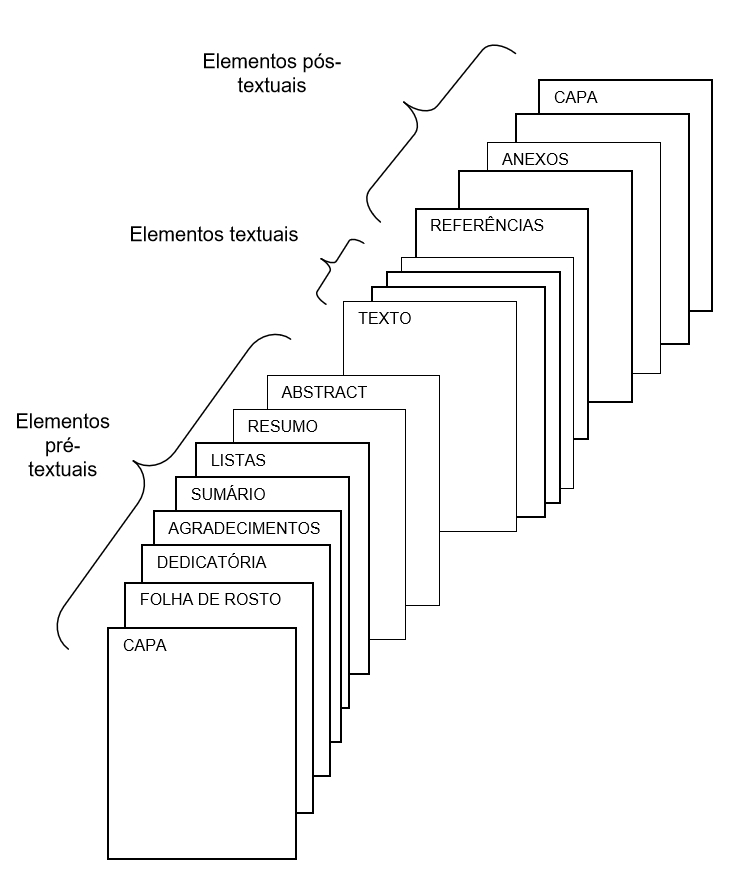
\includegraphics[width=0.7\textwidth]{./cap3/figs/elementos.jpg}
	\caption{Estrutura de um trabalho acadêmico.}
	\label{fig:C3_1}
\end{figure}

As figuras também podem ser agrupadas em conjunto como ilustrado na figura \ref{fig:C3_2}.

\begin{figure}[!t] 
	\centering
	\subfigure[Solução A.]{
		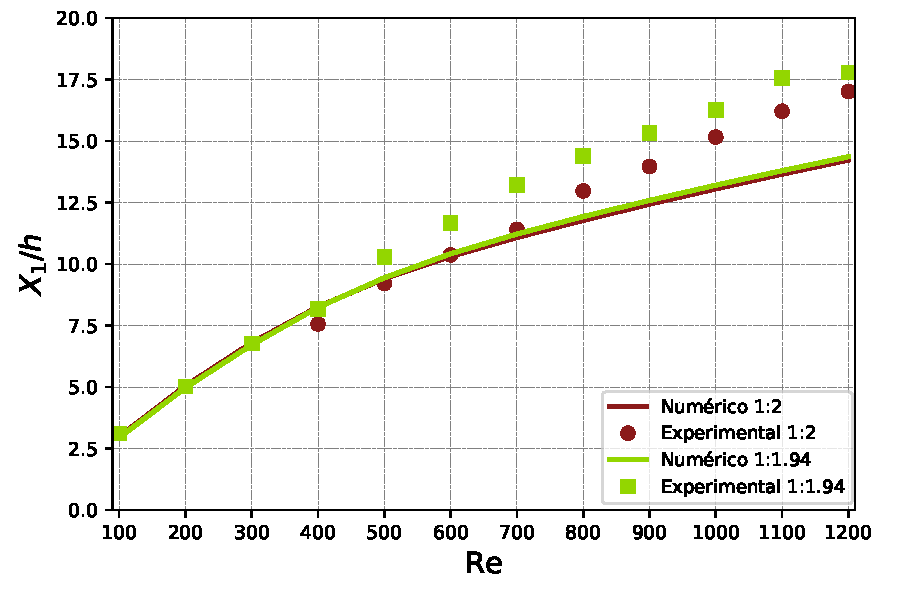
\includegraphics[width=0.45\textwidth]{./cap3/figs/CLAX1.pdf}\label{fig:C3_2a}
	}\hfil
	\subfigure[Solução B.]{
		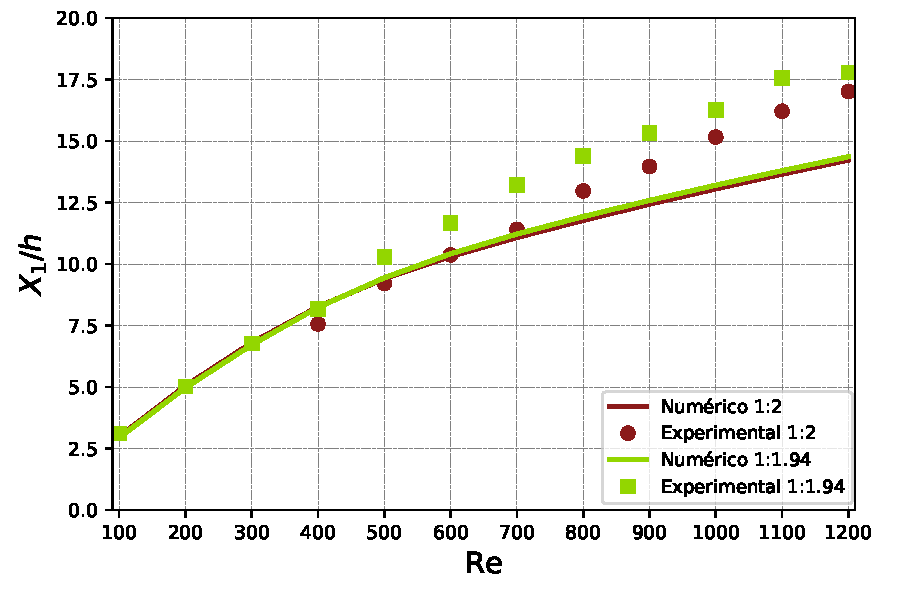
\includegraphics[width=0.45\textwidth]{./cap3/figs/CLAX1.pdf}\label{fig:C3_2b}
	}
	\subfigure[Solução C.]{
		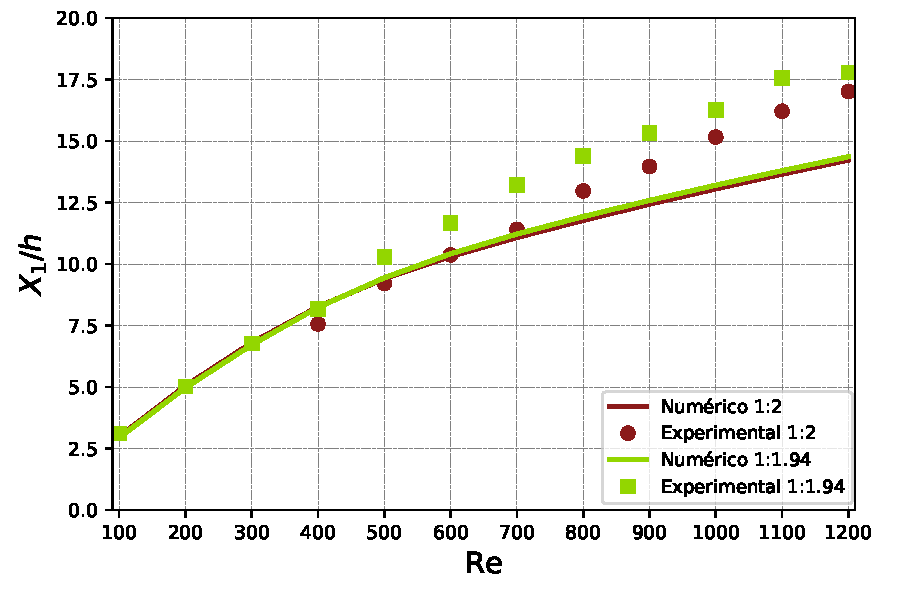
\includegraphics[width=0.45\textwidth]{./cap3/figs/CLAX1.pdf}\label{fig:C3_2c}
	}\hfil
	\subfigure[Solução D.]{
		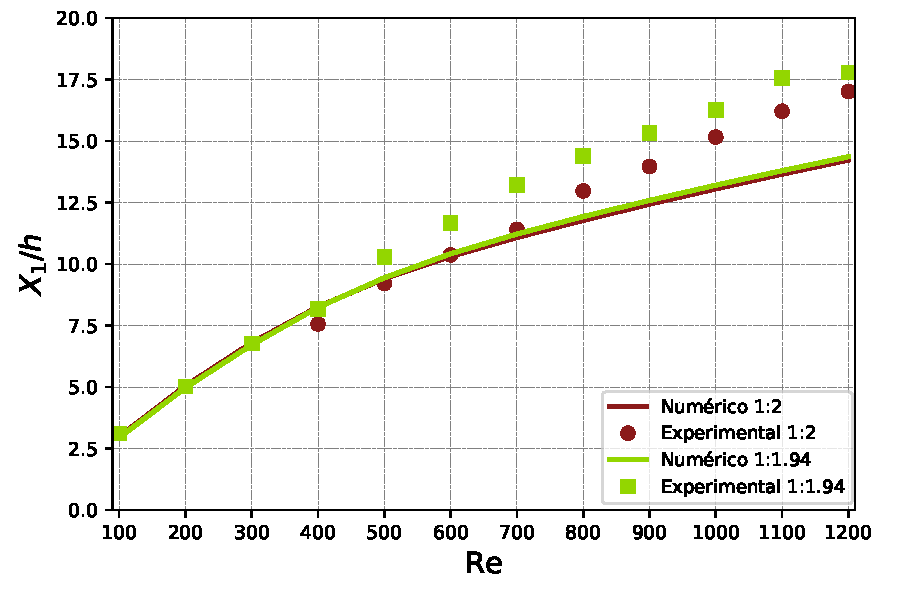
\includegraphics[width=0.45\textwidth]{./cap3/figs/CLAX1.pdf}\label{fig:C3_2d}
	}
	\caption{Exemplo de quatro figuras agrupadas.}
	\label{fig:C3_2}
\end{figure}









